\chapter{Especificació de Requisits}
\label{ch:requisits}

L'especificació de requisits constitueix la base fonamental del projecte \textit{Web Core View}. En tractar-se d'un sistema de gestió per a dispositius de seguretat crítica, la definició de les funcionalitats no només s'ha centrat en l'experiència d'usuari (UX), sinó també en la robustesa de la comunicació asíncrona i el desacoblament entre el maquinari i la interfície.

En aquest capítol es detallen els actors, les històries d'usuari mitjançant la metodologia \textit{Product Backlog}, i l'especificació detallada dels requisits funcionals i no funcionals.

\section{Metodologia d'extracció de requisits}
Els requisits aquí exposats s'han obtingut mitjançant un procés iteratiu amb l'equip d'Embedded de Lanaccess. S'han realitzat sessions d'anàlisi sobre l'aplicació web \textit{legacy} existent --- basada en tecnologies obsoletes com ActiveX --- i entrevistes amb tècnics de camp per identificar els ``punts crítics'' i les limitacions tecnològiques de la plataforma anterior.

\section{Identificació d'actors}
\label{sec:actors}
S'han definit tres actors principals, classificant-los segons el seu nivell d'interacció i privilegis dins del sistema:

\begin{description}
  \item[Administrador de Sistema:] Actor amb privilegis totals sobre el videogravador. El seu objectiu és la posada en marxa de l'equip i el manteniment correctiu. Les seves responsabilitats inclouen:
        \begin{itemize}
          \item Configuració de paràmetres de xarxa (IP, DNS, Gateways).
          \item Gestió del cicle de vida del hardware (Reinicis, actualització de firmware).
          \item Administració de comptes d'usuari i permisos.
        \end{itemize}

  \item[Operador:] Usuari final que utilitza la plataforma per a la monitorització.
        \begin{itemize}
          \item Visualització de vídeo en temps real (\textit{Live}).
          \item Visualització de gravacions històriques.
          \item Supervisió i silenciament d'alarmes en temps real.
        \end{itemize}

  \item[Videogravador (System Actor):] Malgrat ser un element de maquinari, en aquesta arquitectura actua com un usuari actiu que:
        \begin{itemize}
          \item Dicta l'estructura de la interfície mitjançant esquemes JSON.
          \item Notifica esdeveniments de forma proactiva via WebSockets.
          \item Gestiona el control de concurrència per evitar col·lisions de dades.
        \end{itemize}
\end{description}

\section{Històries d'Usuari (User Stories)}
S'utilitzen les \textit{User Stories} per definir el valor que cada funcionalitat aporta a l'usuari final. Cada història inclou els seus criteris d'acceptació.

\subsection{Mòdul de Visualització i Reproducció de Vídeo}
\begin{description}
  \item[\textbf{US-01: Streaming d'alta qualitat}] \hfill \\
        \textbf{Com a} Operador, \textbf{vull} veure el vídeo de qualsevol càmera connectada, \textbf{per tal de} vigilar l'espai protegit en temps real.
        \begin{itemize}
          \item \textit{Criteri 1:} La latència punta a punta ha de ser inferior a 300ms.
          \item \textit{Criteri 2:} El sistema ha de detectar automàticament si el navegador suporta WebRTC o ha de commutar a HLS.
        \end{itemize}

  \item[\textbf{US-02: Gestió de Mosaic}] \hfill \\
        \textbf{Com a} Operador, \textbf{vull} visualitzar fins a 4 càmeres simultàniament, \textbf{per tal de} tenir una visió global de la instal·lació.

  \item[\textbf{US-03: Consulta de gravacions històriques}] \hfill \\
        \textbf{Com a} Operador, \textbf{vull} consultar i reproduir el vídeo gravat del passat mitjançant una línia de temps (\textit{timeline}) gràfica, \textbf{per tal de} revisar incidents de seguretat que s'hagin produït prèviament.
        \begin{itemize}
          \item \textit{Criteri 1:} El reproductor ha de permetre saltar a qualsevol punt temporal passat amb una precisió de 1 segon a través del lliscador de la línia de temps.
          \item \textit{Criteri 2:} La reproducció de vídeo històric s'ha de transmetre mitjançant fragments HLS generats a petició pel gravador.
        \end{itemize}
\end{description}

\subsection{Mòdul de Configuració Dinàmica i Xarxa}
\begin{description}
  \item[\textbf{US-04: Configuració sense recàrrega de codi}] \hfill \\
        \textbf{Com a} Administrador, \textbf{vull} que els nous paràmetres afegits al firmware apareguin a la web sense haver de reprogramar el frontend.
        \begin{itemize}
          \item \textit{Criteri 1:} El frontend ha d'interpretar l'esquema JSON i renderitzar el component visual adequat de forma dinàmica (input, select, slider).
        \end{itemize}

  \item[\textbf{US-05: Configuració de xarxa i IP}] \hfill \\
        \textbf{Com a} Administrador, \textbf{vull} configurar els paràmetres de xarxa del dispositiu (adreça IP, màscara, ports), \textbf{per tal de} garantir la connectivitat del sistema.

  \item[\textbf{US-06: Gestió d'usuaris i permisos}] \hfill \\
        \textbf{Com a} Administrador, \textbf{vull} gestionar els perfils d'usuari i els seus permisos d'accés (grants), \textbf{per tal de} controlar quines accions i vistes pot utilitzar cadascú.
\end{description}

\subsection{Mòdul de Gestió d'Alarmes}
\begin{description}
  \item[\textbf{US-07: Recepció d'alarmes en temps real}] \hfill \\
        \textbf{Com a} Operador, \textbf{vull} rebre notificacions d'alarmes de forma immediata, \textbf{per tal d'}actuar ràpidament davant de qualsevol incidència de seguretat.
        \begin{itemize}
          \item \textit{Criteri 1:} L'alarma s'ha de mostrar a la interfície web en menys d'1 segon des de la seva detecció en el maquinari.
        \end{itemize}

  \item[\textbf{US-08: Configuració de regles d'alarma}] \hfill \\
        \textbf{Com a} Administrador, \textbf{vull} configurar i programar regles de detecció d'alarmes per a cada càmera, \textbf{per tal d'}automatitzar la detecció d'esdeveniments.
\end{description}

\subsection{Mòdul de Manteniment}
\begin{description}
  \item[\textbf{US-09: Consulta i renovació de llicència}] \hfill \\
        \textbf{Com a} Administrador de Sistema, \textbf{vull} consultar l'estat de la llicència del dispositiu i renovar-la quan sigui necessari, \textbf{per tal de} garantir la continuïtat del servei sense interrupcions.

  \item[\textbf{US-10: Actualització de firmware}] \hfill \\
        \textbf{Com a} Administrador de Sistema, \textbf{vull} actualitzar el firmware del dispositiu des de la interfície web, \textbf{per tal de} mantenir el sistema al dia amb les darreres millores i correccions de seguretat.

  \item[\textbf{US-11: Gestió de la configuració del sistema}] \hfill \\
        \textbf{Com a} Administrador, \textbf{vull} restaurar, carregar i descarregar la configuració del dispositiu, \textbf{per tal de} facilitar còpies de seguretat, migracions i recuperació davant de fallades.

  \item[\textbf{US-12: Accés a la documentació del sistema}] \hfill \\
        \textbf{Com a} Administrador de Sistema, \textbf{vull} tenir accés a tota la documentació tècnica del sistema des de la interfície web, \textbf{per tal de} resoldre dubtes i consultar especificacions sense necessitat de recursos externs.

  \item[\textbf{US-13: Descàrrega i consulta de logs}] \hfill \\
        \textbf{Com a} Administrador de Sistema, \textbf{vull} cercar i descarregar els registres d'esdeveniments del sistema, \textbf{per tal de} diagnosticar errors de funcionament o auditar l'ús de la plataforma.
\end{description}

\section{Requisits Funcionals (RF)}
A continuació es detallen els requisits tècnics dividits per blocs funcionals.

\subsection{RF-1: Gestió de l'Accés i Seguretat}
\begin{itemize}
  \item \textbf{RF-1.1 Autenticació:} El sistema ha de validar les credencials contra el servei \textit{Core Legacy}.
  \item \textbf{RF-1.2 Sessió Persistent:} Mantenir la sessió activa mitjançant un mecanisme de \textit{keep-alive} que refresqui la cookie de sessió cada 60 segons.
  \item \textbf{RF-1.3 Control de Concurrència:} El sistema ha de demanar un bloqueig d'escriptura quan un administrador entri en mode edició. Si un altre usuari intenta editar, el sistema mostrarà un avís de ``Només Lectura''.
\end{itemize}

\subsection{RF-2: Visualització Multimèdia}
\begin{itemize}
  \item \textbf{RF-2.1 Protocol WebRTC:} Implementació de la negociació SDP (\textit{Session Description Protocol}) per a vídeo en directe.
  \item \textbf{RF-2.2 Protocol HLS:} Generació de fragments de vídeo per a la reproducció de gravacions històriques i fallback de seguretat.
  \item \textbf{RF-2.3 Línia de Temps Històrica:} Interfície gràfica interactiva per a la cerca i consulta de gravacions passades amb selecció de franja horària.
\end{itemize}

\subsection{RF-3: Motor de Configuració Dinàmica}
Aquest és el requisit funcional més complex i innovador del sistema. El seu principi fonamental és el \textit{schema-driven design}: el gravador dicta l'estructura de la interfície mitjançant esquemes JSON, de manera que el frontend es desacobla completament de la lògica de baix nivell del maquinari.
\begin{itemize}
  \item \textbf{RF-3.1 Interpretació de l'Esquema:} El frontend ha de processar l'esquema JSON rebut del backend i renderitzar dinàmicament el component visual adequat per a cada paràmetre (camp de text, llista desplegable, \textit{slider} numèric). Les restriccions de tipus, rang i format (\textit{regex}) definides a l'esquema s'apliquen automàticament, sense requerir canvis al codi del frontend.
  \item \textbf{RF-3.2 Validació en temps real:} Qualsevol restricció declarada a l'esquema (\texttt{\_min}, \texttt{\_max}, \texttt{\_regex}, \texttt{\_allowedValues}) ha de ser compilada i validada pel motor del frontend abans d'enviar cap petició al backend.
\end{itemize}

\subsection{RF-4: Gestió d'Alarmes}
\begin{itemize}
  \item \textbf{RF-4.1 Recepció en temps real:} El sistema ha de rebre i mostrar les alarmes generades pel maquinari en menys d'1 segon mitjançant una connexió persistent amb el backend.
  \item \textbf{RF-4.2 Historial i filtrat:} El sistema ha de permetre consultar l'historial d'alarmes amb capacitat de filtrat per càmera, rang horari i estat (llegida / no llegida).
  \item \textbf{RF-4.3 Gestió de l'estat:} L'operador ha de poder marcar alarmes individuals com a llegides, arxivar-les o eliminar-les, i qualsevol d'aquestes accions ha de reflectir-se immediatament al backend.
  \item \textbf{RF-4.4 Configuració de regles:} L'administrador ha de poder definir i programar regles de detecció d'alarmes per a cada càmera connectada.
\end{itemize}

\subsection{RF-5: Manteniment i Administració del Sistema}
\begin{itemize}
  \item \textbf{RF-5.1 Registre d'activitat (Log):} El sistema ha de permetre cercar i descarregar els registres d'esdeveniments del dispositiu per facilitar el diagnòstic de fallades i l'auditoria d'ús.
  \item \textbf{RF-5.2 Actualització de firmware:} El sistema ha de gestionar el cicle complet d'actualització del firmware del gravador: pujada del binari, seguiment visual del progrés per fases i detecció automàtica de la tornada en línia del dispositiu un cop reiniciat.
  \item \textbf{RF-5.3 Gestió de la llicència:} El sistema ha de mostrar l'estat actual de la llicència del dispositiu (data de caducitat, funcionalitats habilitades) i permetre iniciar el procés de renovació.
  \item \textbf{RF-5.4 Gestió de la configuració general:} El sistema ha de permetre descarregar la configuració actual del dispositiu, carregar una configuració des d'un fitxer extern i restaurar els valors de fàbrica, amb confirmació explícita de l'usuari en operacions destructives.
  \item \textbf{RF-5.5 Accés a la documentació:} El sistema ha de proporcionar accés integrat a la documentació tècnica oficial del dispositiu (manuals, notes de versió, guies de configuració) sense necessitat de recórrer a recursos externs.
\end{itemize}

\subsection{RF-6: Gestió d'Usuaris i Permisos}
\begin{itemize}
  \item \textbf{RF-6.1 Administració de comptes:} L'administrador ha de poder crear, modificar i eliminar comptes d'usuari del sistema.
  \item \textbf{RF-6.2 Control d'accés basat en rols:} El sistema ha d'aplicar un model de permisos (\textit{grants}) que restringeixi l'accés a mòduls i operacions sensibles en funció del rol assignat a cada usuari.
  \item \textbf{RF-6.3 Canvi de credencials:} El sistema ha de permetre el canvi de contrasenya des de la pròpia interfície web, amb validació de la contrasenya actual.
\end{itemize}

\section{Requisits No Funcionals (RNF)}
Els RNF defineixen les qualitats del sistema i les restriccions tecnològiques.

\subsection{RNF-1: Rendiment i Eficiència}
\begin{itemize}
  \item \textbf{RNF-1.1 Utilització de CPU:} Atès que el videogravador té recursos limitats, s'ha optimitzat el trànsit per evitar el \textit{polling} innecessari, substituint-lo per una arquitectura basada en esdeveniments sobre dos canals WebSocket diferenciats: \textbf{la-core-notifier}, obert de forma persistent des del login per a notificacions globals del sistema, i \textbf{la-core-alarm}, actiu exclusivament a la pàgina d'alarmes per a esdeveniments de detecció en temps real.
  \item \textbf{RNF-1.2 Angular Signals:} La reactivitat de la interfície s'ha de basar en \textit{Angular Signals} per minimitzar les operacions de \textit{Zone.js} i evitar la renderització repetida innecessària del DOM, especialment crític amb vídeos actius.
\end{itemize}

\subsection{RNF-2: Robustesa i Disponibilitat}
\begin{itemize}
  \item \textbf{RNF-2.1 Tolerància a talls de xarxa:} El WebSocket ha d'intentar una reconnexió exponencial (re-try) en cas de pèrdua de connectivitat.
  \item \textbf{RNF-2.2 Fallback de Vídeo:} Si el port WebRTC (UDP 10000-20000) està bloquejat per firewall, el reproductor ha de commutar a HLS en menys de 5 segons.
  \item \textbf{RNF-2.3 Concurrència i Integritat:} Per garantir la consistència de les dades del sistema i evitar escriptures concurrents conflictives entre diferents usuaris administradors, s'exigeix un mecanisme de bloqueig pessimista (\textit{Pessimistic Locking}) en l'adquisició dels formularis de configuració activa. Cap usuari podrà modificar paràmetres del sistema si un altre usuari posseeix el \textit{lock} exclusiu d'aquell mòdul.
\end{itemize}

\subsection{RNF-3: Compatibilitat i Portabilitat}
\begin{itemize}
  \item \textbf{RNF-3.1 Multi-navegador:} Compatible amb les darreres dues versions de Google Chrome, Mozilla Firefox i Microsoft Edge.
  \item \textbf{RNF-3.2 Responsive Design:} La interfície ha de ser plenament operativa en resolucions des de 1024px d'amplada (tauletes de manteniment) fins a 4K (centres de control).
\end{itemize}

\section{Casos d'Ús detallats}
Per aprofundir en la funcionalitat del sistema, es presenta el diagrama de casos d'ús general (Figura \ref{fig:diagrama_casos_us}) i l'especificació detallada dels fluxos crítics.

\begin{figure}[htbp]
  \centering
  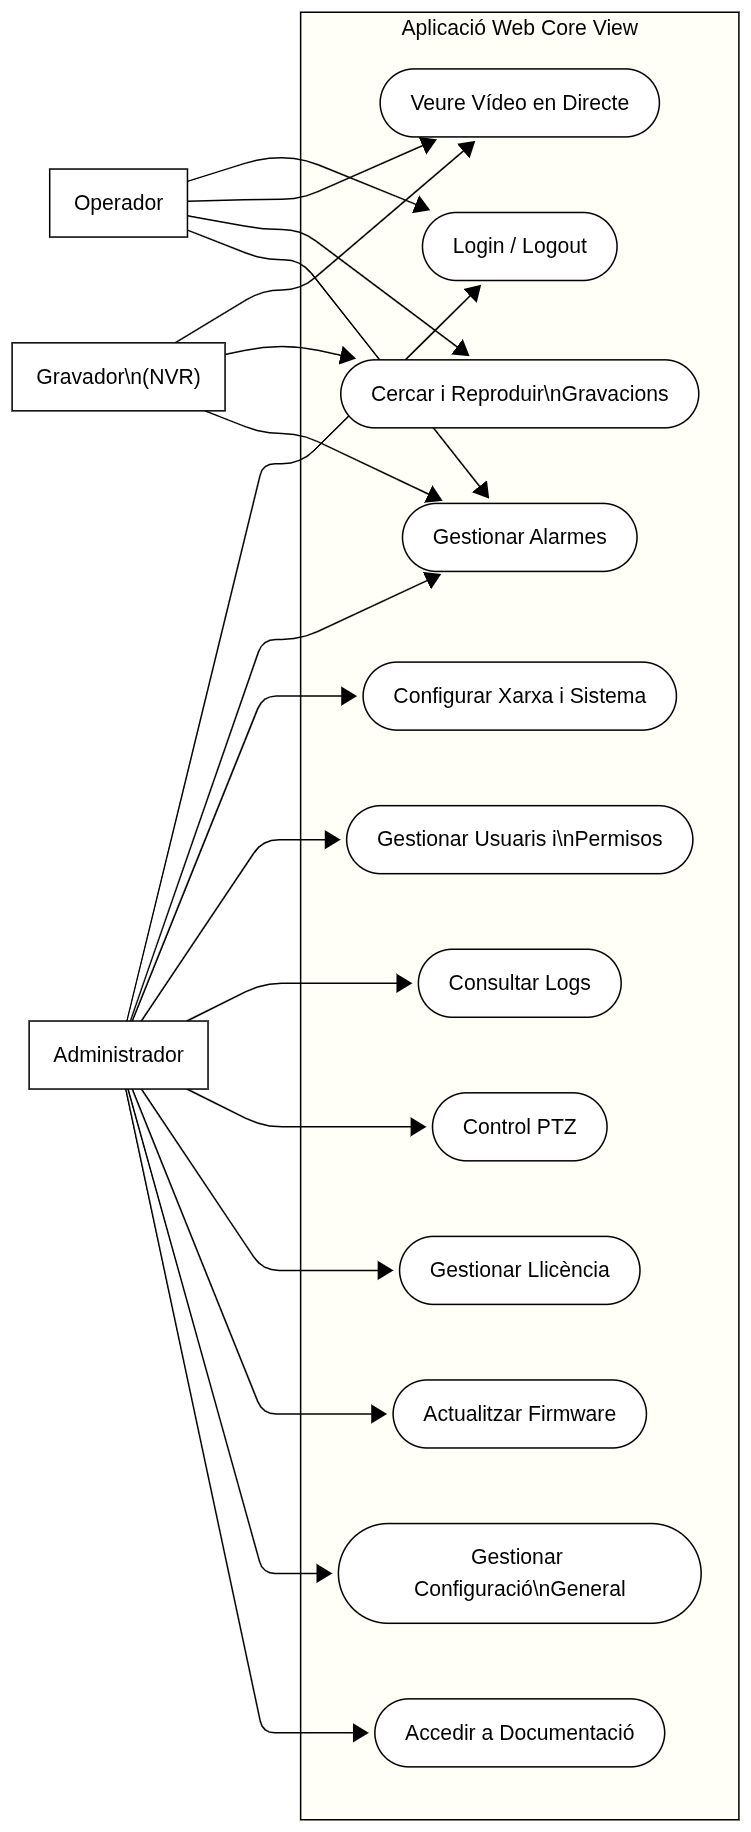
\includegraphics[width=0.9\textwidth, height=0.85\textheight, keepaspectratio]{figures/diagrames/use_cases.png}
  \caption{Diagrama UML de Casos d'Ús.}
  \label{fig:diagrama_casos_us}
  \small Font: Elaboració pròpia.
\end{figure}

\clearpage
\subsection{UC-00: Autenticació i inici de sessió}
L'autenticació és el flux d'entrada obligatori i prerequisit de tots els casos d'ús del sistema.

\begin{table}[htbp]
  \centering
  \small
  \begin{tabular}{|l|p{10cm}|}
    \hline
    \rowcolor{backcolour} \textbf{ID i Nom} & \textbf{UC-00: Autenticació i inici de sessió}                                                                                 \\ \hline
    \textbf{Actor}                          & Administrador / Operador                                                                                                       \\ \hline
    \textbf{Descripció}                     & L'usuari introdueix les seves credencials per obtenir accés al sistema. El procés és en dues fases: primer es validen les credencials i s'estableix la sessió, i després el sistema resol el rol i els permisos de l'usuari.   \\ \hline
    \textbf{Precondicions}                  & El dispositiu NVR és accessible per xarxa. L'usuari disposa de credencials vàlides al sistema.                                 \\ \hline
    \textbf{Flux Principal}                 &
    1. L'usuari accedeix a l'aplicació; el sistema redirigeix a la pàgina d'inici de sessió. \newline
    2. L'usuari introdueix nom d'usuari i contrasenya. \newline
    3. El backend valida les credencials i estableix una cookie de sessió segura, inaccessible des del codi client. \newline
    4. El sistema consulta el perfil de l'usuari per obtenir el seu rol i els permisos associats. \newline
    5. La interfície inicialitza l'estat de sessió i redirigeix a la pàgina principal. \newline
    6. S'estableix un canal de notificacions persistent que roman actiu durant tota la sessió.                                                                                     \\ \hline
    \textbf{Flux Alternatiu}                &
    3a. Si les credencials són incorrectes, el sistema mostra un avís indicant els intents restants. Després de cinc intents fallits consecutius, el compte queda bloquejat temporalment.  \\ \hline
    \textbf{Postcondició}                   & L'usuari té accés a les funcionalitats del sistema d'acord amb el seu rol. La sessió es manté activa mitjançant un mecanisme de refresc periòdic; si el client deixa de respondre durant un temps prolongat, el servidor invalida la sessió automàticament.  \\ \hline
  \end{tabular}
  \caption{Especificació detallada del Cas d'Ús UC-00.}
  \label{tab:uc_login}
\end{table}

\clearpage
\subsection{UC-01: Gestió de l'actualització de firmware}
Aquest cas d'ús és crític per al manteniment del parc de gravadors.

\begin{table}[htbp]
  \centering
  \small
  \begin{tabular}{|l|p{10cm}|}
    \hline
    \rowcolor{backcolour} \textbf{ID i Nom} & \textbf{UC-01: Actualització remota de firmware}                                                                               \\ \hline
    \textbf{Actor}                          & Administrador                                                                                                                  \\ \hline
    \textbf{Descripció}                     & L'usuari carrega un binari de firmware per actualitzar les capacitats del dispositiu.                                          \\ \hline
    \textbf{Precondicions}                  & Usuari autenticat com administrador. El gravador ha de tenir més d'un 10\% d'espai lliure a la partició de sistema.            \\ \hline
    \textbf{Flux Principal}                 &
    1. L'usuari accedeix al mòdul de Manteniment. \newline
    2. L'usuari selecciona un fitxer de firmware des del seu equip local. \newline
    3. El sistema valida la signatura, el format i la mida del fitxer abans de procedir. \newline
    4. S'inicia la transferència del fitxer al dispositiu. La interfície bloqueja totes les accions de configuració i redirigeix qualsevol altre usuari connectat a la pantalla d'actualització. \newline
    5. El sistema mostra el progrés per fases: transferència, gravació a la partició de reserva i reinici. \newline
    6. El dispositiu es reinicia. La interfície mostra una pantalla d'espera fins que el dispositiu torna a estar en línia i confirma que l'actualització s'ha completat correctament.  \\ \hline
    \textbf{Flux Alternatiu}                &
    5a. Si es detecta un error durant la gravació (fitxer corrupte o fallada de verificació), el dispositiu recupera automàticament la versió anterior de firmware i torna a estar operatiu. \\ \hline
    \textbf{Postcondició}                   & El dispositiu funciona amb el nou firmware. La sessió de tots els usuaris es restableix un cop el dispositiu torna a estar en línia.                                               \\ \hline
  \end{tabular}
  \caption{Especificació detallada del Cas d'Ús UC-01.}
  \label{tab:uc_firmware}
\end{table}

\clearpage
\subsection{UC-02: Consulta de gravacions mitjançant Timeline}
\begin{table}[htbp]
  \centering
  \small
  \begin{tabular}{|l|p{10cm}|}
    \hline
    \rowcolor{backcolour} \textbf{ID i Nom} & \textbf{UC-02: Cerca de vídeo històric}              \\ \hline
    \textbf{Actor}                          & Operador                                             \\ \hline
    \textbf{Descripció}                     & L'usuari accedeix al mode de reproducció (\textit{Playback}) per consultar el vídeo gravat en una data i hora concreta, navegant per una línia de temps interactiva generada a partir de l'índex de gravacions del gravador. \\ \hline
    \textbf{Precondicions}                  & Usuari autenticat amb permís de reproducció i descàrrega. El gravador disposa de gravacions per a la data sol·licitada.         \\ \hline
    \textbf{Flux Principal}                 &
    1. L'usuari activa el mode ``Playback'' des de la vista de càmera. \newline
    2. El frontend sol·licita al backend l'índex de gravacions per a una data concreta. \newline
    3. La interfície mostra una línia de temps amb codificació de colors per tipus de gravació (contínua, per alarma). \newline
    4. L'usuari fa clic en un punt de la línia de temps. \newline
    5. El reproductor HLS inicia la càrrega del fragment de vídeo corresponent al punt seleccionat. \\ \hline
    \textbf{Flux Alternatiu}                &
    2a. Si no hi ha gravacions per a la data seleccionada, el sistema informa l'usuari i la línia de temps es mostra buida. \newline
    5a. Si el fragment sol·licitat no és accessible (corrupte o esborrat), el reproductor salta al fragment disponible més proper i n'informa l'usuari. \\ \hline
    \textbf{Postcondició}                   & El reproductor inicia la reproducció del vídeo corresponent al punt seleccionat; l'usuari pot pausar, avançar o retrocedir lliurement. \\ \hline
  \end{tabular}
  \caption{Especificació detallada del Cas d'Ús UC-02.}
\end{table}

\section{Restriccions del sistema}
El desenvolupament s'ha de cenyir a les següents limitacions:
\begin{itemize}
  \item \textbf{Seguretat:} Per evitar atacs \textit{Cross-Site Scripting} (XSS) i \textit{Cross-Site Request Forgery} (CSRF)~\cite{owasp_top10}, no s'utilitzen cookies llegibles per JavaScript ni el \textit{LocalStorage} del navegador per emmagatzemar dades de sessió. La sessió es gestiona mitjançant cookies segures inaccessibles des del codi client, de manera que cap \textit{script} de la pàgina pot llegir ni modificar les credencials. L'estat d'autenticació al \textit{frontend} es manté únicament en memòria.
  \item \textbf{Same-Origin Policy:} Les peticions només poden ser acceptades si provenen del mateix origen que serveix l'aplicació Angular (configurat al NGINX).
  \item \textbf{Llicència:} El sistema ha de verificar que la llicència del hardware permet la visualització de vídeo abans d'obrir els ports de streaming.
\end{itemize}
\section{Marc normatiu i regulacions}
Atesa la naturalesa del projecte, que gestiona fluxos de vídeo en temps real, reproduccions d'imatges de persones físiques i dades de configuració de dispositius de seguretat crítics, el disseny i desenvolupament de \textit{Web Core View} s'ha cenyit als estàndards legals i regulacions tècniques nacionals i europees:

\subsection{Protecció de Dades de Caràcter Personal (RGPD i LOPDGDD)}
El sistema s'adapta al \textbf{Reglament General de Protecció de Dades (RGPD - Reglament UE 2016/679)} \cite{gdpr_reg} i a la legislació de transposició espanyola, la \textbf{Llei Orgànica 3/2018 de Protecció de Dades Personals i Garantia dels Drets Digitals (LOPDGDD)} \cite{lopdgdd_spain}. Especialment, el disseny s'alinea amb l'\textbf{Article 22 de la LOPDGDD}, que regula específicament el tractament d'imatges amb finalitats de videovigilància, sota el principi fonamental de \textbf{Privadesa per Disseny} (\textit{Privacy by Design}):
\begin{itemize}
  \item \textbf{Minimització de dades:} No s'emmagatzemen imatges, captures ni dades personals de forma persistent en el navegador. La sessió d'autenticació no es desa en cap emmagatzematge del client: les cookies de sessió \textit{HttpOnly} les gestiona el servidor NGINX, i l'estat en memòria del \textit{frontend} desapareix en tancar la pestanya o recarregar la pàgina.
  \item \textbf{Seguretat d'accés:} L'accés a les imatges està rígidament controlat per rols d'usuari i privilegis definits en el \textit{backend}, assegurant que només els operadors explícitament autoritzats puguin visualitzar el vídeo en directe i els històrics.
\end{itemize}

\subsection{Seguretat en la comunicació i Xifratge}
Per garantir la integritat i la confidencialitat de les dades, i evitar atacs de tipus interceptació de xarxa, s'obliga a l'ús de protocols criptogràfics segurs:
\begin{itemize}
  \item Totes les peticions a l'API REST es realitzen sota el protocol de transport xifrat \textbf{HTTPS}.
  \item La comunicació asíncrona d'alarmes i notificacions del sistema es realitza mitjançant canals de \textbf{WebSockets Segurs (WSS)}.
  \item La transmissió de fluxos de vídeo WebRTC utilitza xifratge d'extrem a extrem mitjançant el protocol \textbf{DTLS} per al canal de control i \textbf{SRTP} per a la seguretat en els paquets multimèdia.
\end{itemize}

\subsection{Llei de Seguretat Privada i Norma UNE-EN 62676}
El disseny tècnic actua com un element facilitador perquè les entitats de seguretat compleixin amb la \textbf{Llei 5/2014 de Seguretat Privada} a Espanya, així com amb l'estàndard tècnic europeu \textbf{UNE-EN 62676} sobre sistemes de videovigilància per a aplicacions de seguretat:
\begin{itemize}
  \item \textbf{Control de caducitat i esborrat automàtic:} El sistema permet configurar de manera dinàmica les polítiques d'emmagatzematge per garantir que les gravacions se sobreescriuen automàticament en un període màxim de \textbf{30 dies}, en compliment estricte del límit d'emmagatzematge fixat per la Llei de Seguretat Privada i l'Agència Espanyola de Protecció de Dades (AEPD), excepte en cas de requeriment judicial.
  \item \textbf{Registre d'auditoria (Audit Log):} L'aplicació compta amb un servei de registre d'activitat inalterable que monitoritza i audita les accions dels usuaris (qui ha visualitzat quina càmera, en quines dates i hores, i si s'han realitzat descàrregues de vídeo), cosa que assegura la traçabilitat exigida per a la custòdia d'evidències gràfiques.
\end{itemize}
Malgrat aquestes facilitats tècniques, el compliment final de la normativa depèn de la configuració i l'ús real que l'entitat de seguretat privada faci del sistema en la instal·lació del client.

\subsection{Propietat Intel·lectual i Llicències de Programari}

\paragraph{Titularitat del codi.}
El projecte s'ha dut a terme en el marc de la \textbf{Modalitat B} del TFG, que implica el desenvolupament d'un producte real per encàrrec d'una empresa. En virtut de l'\textbf{article 97 del Text Refós de la Llei de Propietat Intel·lectual (LPI)}~\cite{lpi_spain}, els drets d'explotació exclusius d'un programa d'ordinador creat per encàrrec d'una empresa corresponen a aquesta. En conseqüència, el codi font de \textit{Web Core View} és propietat industrial i intel·lectual de \textbf{Lanaccess Telecom, SA}, que n'assumirà el manteniment, l'evolució i la distribució comercial un cop finalitzat el TFG. L'autor conserva els drets morals reconeguts per la LPI i la titularitat acadèmica de la present memòria, que es regeix pel reglament de TFG de la \textbf{Facultat d'Informàtica de Barcelona (FIB)}.

\paragraph{Llicències de les dependències principals.}
El \textit{frontend} de \textit{Web Core View} es construeix sobre programari de codi obert. La Taula~\ref{tab:llicencies} recull les dependències principals i les seves llicències, totes compatibles amb l'ús en productes comercials propietaris i sense cap obligació de publicar el codi font derivat:

\begin{table}[h!]
\centering
\begin{tabular}{lll}
\toprule
\textbf{Dependència} & \textbf{Versió} & \textbf{Llicència} \\
\midrule
Angular (framework)  & 19   & MIT \\
RxJS                 & 7.x  & Apache 2.0 \\
Angular Material     & 19   & MIT \\
ngx-translate        & 16.x & MIT \\
TypeScript           & 5.x  & Apache 2.0 \\
NGINX                & 1.x  & BSD 2-Clause \\
\bottomrule
\end{tabular}
\caption{Llicències de les principals dependències de codi obert de \textit{Web Core View}.}
\label{tab:llicencies}
\end{table}

Cap de les llicències emprades pertany a la família \textit{copyleft} fort (GPL o LGPL en modalitat ``vírica''), de manera que la seva integració en el producte comercial de Lanaccess és legalment conforme i no imposa cap restricció sobre la distribució del \textit{firmware} resultant.